\begin{python}
    self.dashboard <= w.label('Radios', typo='headline4', style=flex_title)
    self.dashboard <= w.radios(
        'Radios',
        options=[[f'chb-{i}', f'chb-{i}'] for i in range(4)],
        on_change=self.on_radios,
        id='my_radios',
    )
    self.dashboard <= w.label(
        f'', id='for_radios', typo=f'body1', style=flex
    )


def on_radios(self):
    value = w.get_value('my_radios')
    document.select_one('#for_radios').html = f'Radios Changed: {value}'
\end{python}


\begin{figure}[H]
\begin{centering}
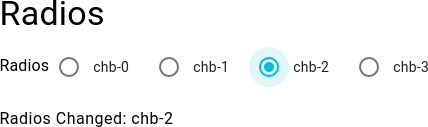
\includegraphics[scale=0.5]{Cap4/Figures/widgets/radios.png}
\par\end{centering}
\caption[Brython Radiant: Radios]{Brython Radiant: Radios.}
\label{fig:radiant_radios}
\end{figure}